% Options for packages loaded elsewhere
\PassOptionsToPackage{unicode}{hyperref}
\PassOptionsToPackage{hyphens}{url}
\PassOptionsToPackage{dvipsnames,svgnames,x11names}{xcolor}
%
\documentclass[
  letterpaper,
  DIV=11,
  numbers=noendperiod]{scrreprt}

\usepackage{amsmath,amssymb}
\usepackage{iftex}
\ifPDFTeX
  \usepackage[T1]{fontenc}
  \usepackage[utf8]{inputenc}
  \usepackage{textcomp} % provide euro and other symbols
\else % if luatex or xetex
  \usepackage{unicode-math}
  \defaultfontfeatures{Scale=MatchLowercase}
  \defaultfontfeatures[\rmfamily]{Ligatures=TeX,Scale=1}
\fi
\usepackage{lmodern}
\ifPDFTeX\else  
    % xetex/luatex font selection
\fi
% Use upquote if available, for straight quotes in verbatim environments
\IfFileExists{upquote.sty}{\usepackage{upquote}}{}
\IfFileExists{microtype.sty}{% use microtype if available
  \usepackage[]{microtype}
  \UseMicrotypeSet[protrusion]{basicmath} % disable protrusion for tt fonts
}{}
\makeatletter
\@ifundefined{KOMAClassName}{% if non-KOMA class
  \IfFileExists{parskip.sty}{%
    \usepackage{parskip}
  }{% else
    \setlength{\parindent}{0pt}
    \setlength{\parskip}{6pt plus 2pt minus 1pt}}
}{% if KOMA class
  \KOMAoptions{parskip=half}}
\makeatother
\usepackage{xcolor}
\setlength{\emergencystretch}{3em} % prevent overfull lines
\setcounter{secnumdepth}{5}
% Make \paragraph and \subparagraph free-standing
\makeatletter
\ifx\paragraph\undefined\else
  \let\oldparagraph\paragraph
  \renewcommand{\paragraph}{
    \@ifstar
      \xxxParagraphStar
      \xxxParagraphNoStar
  }
  \newcommand{\xxxParagraphStar}[1]{\oldparagraph*{#1}\mbox{}}
  \newcommand{\xxxParagraphNoStar}[1]{\oldparagraph{#1}\mbox{}}
\fi
\ifx\subparagraph\undefined\else
  \let\oldsubparagraph\subparagraph
  \renewcommand{\subparagraph}{
    \@ifstar
      \xxxSubParagraphStar
      \xxxSubParagraphNoStar
  }
  \newcommand{\xxxSubParagraphStar}[1]{\oldsubparagraph*{#1}\mbox{}}
  \newcommand{\xxxSubParagraphNoStar}[1]{\oldsubparagraph{#1}\mbox{}}
\fi
\makeatother

\usepackage{color}
\usepackage{fancyvrb}
\newcommand{\VerbBar}{|}
\newcommand{\VERB}{\Verb[commandchars=\\\{\}]}
\DefineVerbatimEnvironment{Highlighting}{Verbatim}{commandchars=\\\{\}}
% Add ',fontsize=\small' for more characters per line
\usepackage{framed}
\definecolor{shadecolor}{RGB}{241,243,245}
\newenvironment{Shaded}{\begin{snugshade}}{\end{snugshade}}
\newcommand{\AlertTok}[1]{\textcolor[rgb]{0.68,0.00,0.00}{#1}}
\newcommand{\AnnotationTok}[1]{\textcolor[rgb]{0.37,0.37,0.37}{#1}}
\newcommand{\AttributeTok}[1]{\textcolor[rgb]{0.40,0.45,0.13}{#1}}
\newcommand{\BaseNTok}[1]{\textcolor[rgb]{0.68,0.00,0.00}{#1}}
\newcommand{\BuiltInTok}[1]{\textcolor[rgb]{0.00,0.23,0.31}{#1}}
\newcommand{\CharTok}[1]{\textcolor[rgb]{0.13,0.47,0.30}{#1}}
\newcommand{\CommentTok}[1]{\textcolor[rgb]{0.37,0.37,0.37}{#1}}
\newcommand{\CommentVarTok}[1]{\textcolor[rgb]{0.37,0.37,0.37}{\textit{#1}}}
\newcommand{\ConstantTok}[1]{\textcolor[rgb]{0.56,0.35,0.01}{#1}}
\newcommand{\ControlFlowTok}[1]{\textcolor[rgb]{0.00,0.23,0.31}{\textbf{#1}}}
\newcommand{\DataTypeTok}[1]{\textcolor[rgb]{0.68,0.00,0.00}{#1}}
\newcommand{\DecValTok}[1]{\textcolor[rgb]{0.68,0.00,0.00}{#1}}
\newcommand{\DocumentationTok}[1]{\textcolor[rgb]{0.37,0.37,0.37}{\textit{#1}}}
\newcommand{\ErrorTok}[1]{\textcolor[rgb]{0.68,0.00,0.00}{#1}}
\newcommand{\ExtensionTok}[1]{\textcolor[rgb]{0.00,0.23,0.31}{#1}}
\newcommand{\FloatTok}[1]{\textcolor[rgb]{0.68,0.00,0.00}{#1}}
\newcommand{\FunctionTok}[1]{\textcolor[rgb]{0.28,0.35,0.67}{#1}}
\newcommand{\ImportTok}[1]{\textcolor[rgb]{0.00,0.46,0.62}{#1}}
\newcommand{\InformationTok}[1]{\textcolor[rgb]{0.37,0.37,0.37}{#1}}
\newcommand{\KeywordTok}[1]{\textcolor[rgb]{0.00,0.23,0.31}{\textbf{#1}}}
\newcommand{\NormalTok}[1]{\textcolor[rgb]{0.00,0.23,0.31}{#1}}
\newcommand{\OperatorTok}[1]{\textcolor[rgb]{0.37,0.37,0.37}{#1}}
\newcommand{\OtherTok}[1]{\textcolor[rgb]{0.00,0.23,0.31}{#1}}
\newcommand{\PreprocessorTok}[1]{\textcolor[rgb]{0.68,0.00,0.00}{#1}}
\newcommand{\RegionMarkerTok}[1]{\textcolor[rgb]{0.00,0.23,0.31}{#1}}
\newcommand{\SpecialCharTok}[1]{\textcolor[rgb]{0.37,0.37,0.37}{#1}}
\newcommand{\SpecialStringTok}[1]{\textcolor[rgb]{0.13,0.47,0.30}{#1}}
\newcommand{\StringTok}[1]{\textcolor[rgb]{0.13,0.47,0.30}{#1}}
\newcommand{\VariableTok}[1]{\textcolor[rgb]{0.07,0.07,0.07}{#1}}
\newcommand{\VerbatimStringTok}[1]{\textcolor[rgb]{0.13,0.47,0.30}{#1}}
\newcommand{\WarningTok}[1]{\textcolor[rgb]{0.37,0.37,0.37}{\textit{#1}}}

\providecommand{\tightlist}{%
  \setlength{\itemsep}{0pt}\setlength{\parskip}{0pt}}\usepackage{longtable,booktabs,array}
\usepackage{calc} % for calculating minipage widths
% Correct order of tables after \paragraph or \subparagraph
\usepackage{etoolbox}
\makeatletter
\patchcmd\longtable{\par}{\if@noskipsec\mbox{}\fi\par}{}{}
\makeatother
% Allow footnotes in longtable head/foot
\IfFileExists{footnotehyper.sty}{\usepackage{footnotehyper}}{\usepackage{footnote}}
\makesavenoteenv{longtable}
\usepackage{graphicx}
\makeatletter
\newsavebox\pandoc@box
\newcommand*\pandocbounded[1]{% scales image to fit in text height/width
  \sbox\pandoc@box{#1}%
  \Gscale@div\@tempa{\textheight}{\dimexpr\ht\pandoc@box+\dp\pandoc@box\relax}%
  \Gscale@div\@tempb{\linewidth}{\wd\pandoc@box}%
  \ifdim\@tempb\p@<\@tempa\p@\let\@tempa\@tempb\fi% select the smaller of both
  \ifdim\@tempa\p@<\p@\scalebox{\@tempa}{\usebox\pandoc@box}%
  \else\usebox{\pandoc@box}%
  \fi%
}
% Set default figure placement to htbp
\def\fps@figure{htbp}
\makeatother

\KOMAoption{captions}{tableheading}
\makeatletter
\@ifpackageloaded{tcolorbox}{}{\usepackage[skins,breakable]{tcolorbox}}
\@ifpackageloaded{fontawesome5}{}{\usepackage{fontawesome5}}
\definecolor{quarto-callout-color}{HTML}{909090}
\definecolor{quarto-callout-note-color}{HTML}{0758E5}
\definecolor{quarto-callout-important-color}{HTML}{CC1914}
\definecolor{quarto-callout-warning-color}{HTML}{EB9113}
\definecolor{quarto-callout-tip-color}{HTML}{00A047}
\definecolor{quarto-callout-caution-color}{HTML}{FC5300}
\definecolor{quarto-callout-color-frame}{HTML}{acacac}
\definecolor{quarto-callout-note-color-frame}{HTML}{4582ec}
\definecolor{quarto-callout-important-color-frame}{HTML}{d9534f}
\definecolor{quarto-callout-warning-color-frame}{HTML}{f0ad4e}
\definecolor{quarto-callout-tip-color-frame}{HTML}{02b875}
\definecolor{quarto-callout-caution-color-frame}{HTML}{fd7e14}
\makeatother
\makeatletter
\@ifpackageloaded{bookmark}{}{\usepackage{bookmark}}
\makeatother
\makeatletter
\@ifpackageloaded{caption}{}{\usepackage{caption}}
\AtBeginDocument{%
\ifdefined\contentsname
  \renewcommand*\contentsname{Table of contents}
\else
  \newcommand\contentsname{Table of contents}
\fi
\ifdefined\listfigurename
  \renewcommand*\listfigurename{List of Figures}
\else
  \newcommand\listfigurename{List of Figures}
\fi
\ifdefined\listtablename
  \renewcommand*\listtablename{List of Tables}
\else
  \newcommand\listtablename{List of Tables}
\fi
\ifdefined\figurename
  \renewcommand*\figurename{Figure}
\else
  \newcommand\figurename{Figure}
\fi
\ifdefined\tablename
  \renewcommand*\tablename{Table}
\else
  \newcommand\tablename{Table}
\fi
}
\@ifpackageloaded{float}{}{\usepackage{float}}
\floatstyle{ruled}
\@ifundefined{c@chapter}{\newfloat{codelisting}{h}{lop}}{\newfloat{codelisting}{h}{lop}[chapter]}
\floatname{codelisting}{Listing}
\newcommand*\listoflistings{\listof{codelisting}{List of Listings}}
\makeatother
\makeatletter
\makeatother
\makeatletter
\@ifpackageloaded{caption}{}{\usepackage{caption}}
\@ifpackageloaded{subcaption}{}{\usepackage{subcaption}}
\makeatother

\usepackage{bookmark}

\IfFileExists{xurl.sty}{\usepackage{xurl}}{} % add URL line breaks if available
\urlstyle{same} % disable monospaced font for URLs
\hypersetup{
  pdftitle={Introduction to R},
  pdfauthor={Daulton Selke},
  colorlinks=true,
  linkcolor={blue},
  filecolor={Maroon},
  citecolor={Blue},
  urlcolor={Blue},
  pdfcreator={LaTeX via pandoc}}


\title{Introduction to R}
\usepackage{etoolbox}
\makeatletter
\providecommand{\subtitle}[1]{% add subtitle to \maketitle
  \apptocmd{\@title}{\par {\large #1 \par}}{}{}
}
\makeatother
\subtitle{SOC 300: Social Research Methods}
\author{Daulton Selke}
\date{2025-09-05}

\begin{document}
\maketitle

\renewcommand*\contentsname{Table of contents}
{
\hypersetup{linkcolor=}
\setcounter{tocdepth}{2}
\tableofcontents
}

\bookmarksetup{startatroot}

\chapter*{Preface}\label{preface}
\addcontentsline{toc}{chapter}{Preface}

\markboth{Preface}{Preface}

Welcome to this introductory R tutorial for SOC 300!

Here you will find all the step-by-step instructions for completing our
initial foray into R for quantitative analysis of social science data.
We will begin by establishing some common ground in basic R operations
and functionality. After we lay this foundation, we will progress
through various data processing tasks---from importing and cleaning
public data to visualizing and analyzing these data for consumption by
interested stakeholders.

You will receive an R script file with the commands detailed here, so
that you can easily run and manipulate them on your own device, but you
will always be able to refer to this mini-textbook in the event that you
would like to see everything in one place and refer to some more
detailed documentation on various R operations.

\part{Day 1: Getting Started}

\chapter{Background}\label{background}

Before we start exploring some of R's basic functionality, I'm going to
set the stage a little on what R and R studio are, why we are using
these tools in particular, and what we will need to know before we dig
in.

\section{What is R?}\label{what-is-r}

At it's core, R is a programming language. There's a lot to say about
this from a computer science perspective, but, for our purposes, you can
just think of R as a language with a very particular structure that's
designed to tell our computers what to do.

There are all sorts of different programming languages out there, and
they all offer certain benefits or cater to particular computing needs.
Unlike some general purpose languages like C, C++, or Python, R is
relatively specialized, and this is part of what makes it so useful for
us. R is designed with statistical computing as a primary motivator, and
now---roughly 30 years into its tenure---stands as one of the most
widely adopted resources for statistical data science in the social
sciences and beyond.

Though there can be a bit of a learning curve when getting used to R, we
will focus on exactly the things that we need and build ourselves up
slowly. Once you get used to it, R will allow you to perform incredibly
complex statistical procedures with relative ease, and it can even help
us with other related tasks like visualizing and presenting our
analyses.

\section{What is R Studio?}\label{what-is-r-studio}

We are going to pair R with the software R Studio, which is what's known
as an Integrated Development Environment (IDE). Programming languages
can be leveraged in a number of different ways. You could run R commands
entirely from a Windows command line or Mac terminal. But that would
probably not be very ideal for us---not to mention sort of ethereal and
frustrating for those of without any programming experience. IDEs
provide user-friendly interfaces for working with programming languages,
so that we can easily manage our code, quickly generate and view the
output of our analyses, and generally keep track of what we are doing
with R. There are lots of other IDEs out there, but R Studio is an ideal
balance of ease and power, so it will serve as our IDE of choice.

The best way to think about R Studio's relationship to R is by framing
it as an analogy with a desktop computer. R Studio is to R as a monitor
is to a computer. R is the thing that's doing all the heavy lifting
computationally, and R Studio is the thing that allows us to view and
interact with R in a way that's simple and straightforward.

\section{Acquiring R and R Studio}\label{acquiring-r-and-r-studio}

All of the CHASS computers (and likely most NC State computers) come
with R and R Studio, so you do not need to download them, but you may
find it convenient to work on R assignments using your own personal
device, so I've provided some instructions below.

Note that you will want to install R first,

\subsection{Downloading R}\label{downloading-r}

You can download R from the
\href{https://www.r-project.org/}{Comprehensive R Archive Network
(CRAN)}.

When you click that link, you will arrive at CRAN's homepage. Navigate
to the sidebar on the left, find `Download' near the top, and then click
`CRAN'. This will take you to the `mirrors' page. Mirrors are just
different host locations for downloading the R installation files. This
allows you to maximize download speed by choosing a nearby server, so
scroll down to `USA' and choose one of those (I usually opt for the
Durham, NC mirror).

Unless you are very experienced with computers, you should download one
of the options listed as `pre-compiled binary distributions'. These will
typically be the first options listed. Don't even worry about what that
means if you're not familiar. Just choose the one that reflects your
operating system (there are options for Windows, Mac, and Linux) That
should download an R installer, and you can follow the directions to
complete a default installation.

\subsection{Downloading R Studio}\label{downloading-r-studio}

R Studio is a little more straightforward to download. Just
\href{https://posit.co/download/rstudio-desktop/}{navigate to its
homepage}, scroll down a little, and you will find a big button that
says `Download R Studio for {[}your operating system{]}'. Go ahead and
run the installer with the default settings.

\chapter{R Fundamentals}\label{r-fundamentals}

\section{Basic Operations}\label{basic-operations}

First, we will start by exploring some of the basic characteristics of
R.

R can be used as a simple calculator and will process both numbers and
conventional mathematical operator symbols. You can run the commands
below by placing your cursor at the beginning or end of the line and
pressing CTRL+Enter (Windows) or Command+Return (Mac)

\begin{Shaded}
\begin{Highlighting}[]
\DecValTok{5}\SpecialCharTok{+}\DecValTok{2}
\end{Highlighting}
\end{Shaded}

\begin{verbatim}
[1] 7
\end{verbatim}

You should see the result displayed in the console below.

\section{Storing Objects}\label{storing-objects}

R is especially helpful for allowing us to create and store objects that
we can call and manipulate later. We can create names for these objects
and then use R's `assignment operator,' the \texttt{\textless{}-}
symbol, to assign a value to our specified object name. Here, we'll
assign the previous calculation to an object that we are calling
\texttt{our\_object}.

If you run this command on your own device, you should see
\texttt{our\_object} populate in the upper-right Environment window.
This is where you can find all of the objects that you create in your R
session. We can run the object itself, as well as combine it with other
operations

\begin{Shaded}
\begin{Highlighting}[]
\NormalTok{our\_object }\OtherTok{\textless{}{-}} \DecValTok{5}\SpecialCharTok{+}\DecValTok{2}
\end{Highlighting}
\end{Shaded}

There are some more baroque ways around this, but it's best to operate
under the impression that object names cannot include spaces (or start
with numbers). This kind of thing is common in some programming
languages, so there are a couple stylistic conventions to address this.
I tend to use what's called `snake case,' which involves replacing
spaces with underscores. There's also `camel case,' where each word has
the first letter capitalized, e.g.~MyVariableName. I would settle on one
that you like and be consistent with it.

\begin{Shaded}
\begin{Highlighting}[]
\NormalTok{our\_object}
\end{Highlighting}
\end{Shaded}

\begin{verbatim}
[1] 7
\end{verbatim}

\begin{Shaded}
\begin{Highlighting}[]
\NormalTok{our\_object }\SpecialCharTok{+} \DecValTok{3}
\end{Highlighting}
\end{Shaded}

\begin{verbatim}
[1] 10
\end{verbatim}

\begin{Shaded}
\begin{Highlighting}[]
\NormalTok{our\_object }\SpecialCharTok{*} \DecValTok{100}
\end{Highlighting}
\end{Shaded}

\begin{verbatim}
[1] 700
\end{verbatim}

\section{A Note on Functions}\label{a-note-on-functions}

R is also useful for its implementation of functions, which you can
think of in the sense you likely learned in your math classes. Functions
are defined procedures that take some input value, transform that value
according to the procedure, and then output a new value.

R comes with a great deal of already defined functions, and we can use
these to perform all sorts of helpful operations. You can call a
function by indicating it's common name and then placing it's required
inputs between parentheses, e.g.~\texttt{function\_name(input)}.Note
that function inputs are also often referred to as `arguments'. We'll
get a lot of mileage out of functions, and part of the initial learning
curve of R will be related to getting used to the range of available
functions and the syntax you must follow to call them.

Now, let's take a step back and think about some of our basic building
blocks in R.

\section{Vectors and R Data Types}\label{vectors-and-r-data-types}

You can think of vectors as ordered sets of values. We can use the
\texttt{c()} function (short for `combine') to create a vector made up
of the values we provide. Let's make a few different vectors

\begin{Shaded}
\begin{Highlighting}[]
\NormalTok{num\_vec }\OtherTok{\textless{}{-}} \FunctionTok{c}\NormalTok{(}\FloatTok{1.2}\NormalTok{, }\FloatTok{3.4}\NormalTok{, }\FloatTok{5.6}\NormalTok{, }\FloatTok{7.1}\NormalTok{, }\FloatTok{2.8}\NormalTok{)}

\NormalTok{character\_vec }\OtherTok{\textless{}{-}} \FunctionTok{c}\NormalTok{(}\StringTok{"east"}\NormalTok{, }\StringTok{"west"}\NormalTok{, }\StringTok{"south"}\NormalTok{, }\StringTok{"south"}\NormalTok{, }\StringTok{"north"}\NormalTok{) }

\NormalTok{logical\_vec }\OtherTok{\textless{}{-}} \FunctionTok{c}\NormalTok{(}\ConstantTok{TRUE}\NormalTok{, }\ConstantTok{FALSE}\NormalTok{, }\ConstantTok{TRUE}\NormalTok{, }\ConstantTok{FALSE}\NormalTok{, }\ConstantTok{FALSE}\NormalTok{) }
\end{Highlighting}
\end{Shaded}

Let's talk a bit about what we have here. Each of these vectors
represents a \textbf{data type} in R, or, in other words, one of the
basic ways in which R stores data. There are some more data types out
there that we may encounter, but these are the most most relevant for
us.

\begin{itemize}
\item
  \textbf{\emph{Numeric Data:}} As the name suggests, this is the
  typical fashion in which numbers are stored in R. Numeric data
  encompasses both \emph{continuous} values and \emph{discrete} values.
  These are essentially numbers that can have decimal places
  vs.~integers (whole numbers).
\item
  \textbf{\emph{Character Data:}} Character here refers to the idea of
  character strings. This is typically how R stores text data---as
  distinct strings of text. Note that, while numbers are typically
  processed as numeric by R, numbers can also become character data if
  you place them between quotation marks. Some wonky things can
  occasionally happen when you are importing data in from various source
  file types as well (e.g.~.CSV, .XLSX, etc.)
\item
  \textbf{\emph{Logical Data:}} In R syntax, upper-case `true' and
  `false' have fixed values in R and, when used without quotes, will
  refer to these pre-defined logical values. We probably won't use this
  data type much for analyses, but we will run into them in other
  places. They can be useful for sorting and searching through subsets
  of data, and we will also use logical values to turn certain
  procedures on or off in some functions.
\end{itemize}

Many R functions will respond differently to different data types, so
it's important to keep these in mind when you need to troubleshoot
errors.

Take the \texttt{mean()} function, for example. As the name implies,
this function will return the arithmetic mean of a numeric vector. Let's
give it the one we just made above:

\begin{Shaded}
\begin{Highlighting}[]
\FunctionTok{mean}\NormalTok{(num\_vec)}
\end{Highlighting}
\end{Shaded}

\begin{verbatim}
[1] 4.02
\end{verbatim}

\begin{Shaded}
\begin{Highlighting}[]
\NormalTok{(}\FloatTok{1.2+3.4+5.6+7.1+2.8}\NormalTok{)}\SpecialCharTok{/}\DecValTok{5}
\end{Highlighting}
\end{Shaded}

\begin{verbatim}
[1] 4.02
\end{verbatim}

Note that it gives the same response as if we had manually calculated
it. Functions can make our lives a lot easier with larger amounts of
data, but always make sure you're familiar with what's going on under
the hood of any given function.

But, what happens when we run the following command?

\begin{Shaded}
\begin{Highlighting}[]
\FunctionTok{mean}\NormalTok{(character\_vec)}
\end{Highlighting}
\end{Shaded}

\begin{verbatim}
Warning in mean.default(character_vec): argument is not numeric or logical:
returning NA
\end{verbatim}

\begin{verbatim}
[1] NA
\end{verbatim}

It doesn't make any sense to take the mean of the cardinal directions,
so it will throw a warning message. We need a variable that can be
represented numerically. Note that \texttt{mean()} also accepts logical
variables, as, in R, TRUEs will be counted as 1s and FALSEs will be
counted as 0s. In this case, you will be getting the proportion of true
responses

\begin{Shaded}
\begin{Highlighting}[]
\FunctionTok{mean}\NormalTok{(logical\_vec)}
\end{Highlighting}
\end{Shaded}

\begin{verbatim}
[1] 0.4
\end{verbatim}

\begin{Shaded}
\begin{Highlighting}[]
\NormalTok{(}\DecValTok{1}\SpecialCharTok{+}\DecValTok{0}\SpecialCharTok{+}\DecValTok{1}\SpecialCharTok{+}\DecValTok{0}\SpecialCharTok{+}\DecValTok{0}\NormalTok{)}\SpecialCharTok{/}\DecValTok{5}
\end{Highlighting}
\end{Shaded}

\begin{verbatim}
[1] 0.4
\end{verbatim}

Now that we've talked about some of these basic building blocks for
data, let's talk about putting them together.

\section{Data Frames}\label{data-frames}

For the most part, we will be working with data frames. These are
collections of data organized in rows and columns. In data science, it's
generally preferable for data to take a particular shape wherein each
row indicates a single observation, and each column represents a unique
variable. This is called the `tidy' data format.

Let's use the vectors we created above to mock up a little data frame.
We will imagine some variables that those vectors could represent.
First, let's make a couple more vectors.

We want a data frame that reflects the `tidy' format (rows =
observations, columns = variables). So, let's add a character vector of
participant IDs associated with imaginary people in our mock data set.
For reasons that will become clear in the next section, we are also
going to add another character vector.

\begin{Shaded}
\begin{Highlighting}[]
\NormalTok{p\_id\_vec}\OtherTok{\textless{}{-}}\FunctionTok{c}\NormalTok{(}\StringTok{"p1"}\NormalTok{, }\StringTok{"p2"}\NormalTok{, }\StringTok{"p3"}\NormalTok{, }\StringTok{"p4"}\NormalTok{, }\StringTok{"p5"}\NormalTok{)}

\NormalTok{ordinal\_vec}\OtherTok{\textless{}{-}}\FunctionTok{c}\NormalTok{(}\StringTok{"small"}\NormalTok{, }\StringTok{"medium"}\NormalTok{, }\StringTok{"medium"}\NormalTok{, }\StringTok{"large"}\NormalTok{, }\StringTok{"medium"}\NormalTok{)}
\end{Highlighting}
\end{Shaded}

Now, let's use a base R function to create a data frame and assign it to
a new object.

We can use the \texttt{data.frame()} function to build up our data
frame. This function expects that we will give it some vectors, which it
will organize into columns. We could just give it the vectors, and it
will take the vector names as column names, e.g.:

\begin{Shaded}
\begin{Highlighting}[]
\NormalTok{our\_df }\OtherTok{\textless{}{-}} \FunctionTok{data.frame}\NormalTok{(p\_id\_vec, num\_vec, character\_vec, ordinal\_vec, logical\_vec)}
\end{Highlighting}
\end{Shaded}

or we can specify new variable names and use the \texttt{=} sign to
associate them with the vector. We will go with this latter strategy
because our current vector names do not translate well to variable
names.

We'll go ahead and imagine building a small data frame of dog owners and
rename our vectors accordingly.

\begin{Shaded}
\begin{Highlighting}[]
\NormalTok{our\_df}\OtherTok{\textless{}{-}}\FunctionTok{data.frame}\NormalTok{(}
  \AttributeTok{p\_id =}\NormalTok{ p\_id\_vec,}
  \AttributeTok{dog\_size =}\NormalTok{ ordinal\_vec,}
  \AttributeTok{side\_of\_town =}\NormalTok{ character\_vec,}
  \AttributeTok{food\_per\_day =}\NormalTok{ num\_vec, }
  \AttributeTok{has\_a\_labrador =}\NormalTok{ logical\_vec}
\NormalTok{)}
\end{Highlighting}
\end{Shaded}

\begin{tcolorbox}[enhanced jigsaw, breakable, leftrule=.75mm, toprule=.15mm, colbacktitle=quarto-callout-tip-color!10!white, opacityback=0, titlerule=0mm, coltitle=black, colback=white, opacitybacktitle=0.6, left=2mm, bottomtitle=1mm, bottomrule=.15mm, toptitle=1mm, colframe=quarto-callout-tip-color-frame, arc=.35mm, rightrule=.15mm, title=\textcolor{quarto-callout-tip-color}{\faLightbulb}\hspace{0.5em}{Tip}]

As a slight tangent, note that we can use line breaks to our advantage
with longer strings of code. The above command is identical to the one
below, but some find the line-break strategy more intuitively readable.
It's most important that your code works, so you don't have to organize
it like that, but know that's an option

\begin{Shaded}
\begin{Highlighting}[]
\NormalTok{our\_df }\OtherTok{\textless{}{-}} \FunctionTok{data.frame}\NormalTok{(}\AttributeTok{p\_id =}\NormalTok{ p\_id\_vec, }\AttributeTok{dog\_size =}\NormalTok{ ordinal\_vec, }\AttributeTok{side\_of\_town =}\NormalTok{ character\_vec, }\AttributeTok{food\_per\_day =}\NormalTok{ num\_vec, }\AttributeTok{has\_a\_labrador =}\NormalTok{ logical\_vec)}
\end{Highlighting}
\end{Shaded}

\end{tcolorbox}

Now our vectors make up meaningful variables in our mock data frame.

\begin{itemize}
\tightlist
\item
  \texttt{p\_id} = An ID for each participant in our survey of dog
  owners
\item
  \texttt{dog\_size} = Owner's ranking of their dog's size
\item
  \texttt{side\_of\_town} = Which part of town the owners reside
\item
  \texttt{food\_per\_day} = The amount of food each owner feeds their
  dog daily (in ounces)
\item
  \texttt{has\_a\_labrador} = true/false indicator for whether the owner
  has a lab or not
\end{itemize}

Take a look at our new data frame by clicking on the object in our
Environment window at the upper right, or by running the command
\texttt{View(our\_df)}.

Once we have created a data frame, we can refer to individual variable
vectors with the \texttt{\$} operator in R

\begin{Shaded}
\begin{Highlighting}[]
\NormalTok{our\_df}\SpecialCharTok{$}\NormalTok{food\_per\_day}
\end{Highlighting}
\end{Shaded}

\begin{verbatim}
[1] 1.2 3.4 5.6 7.1 2.8
\end{verbatim}

\begin{Shaded}
\begin{Highlighting}[]
\FunctionTok{mean}\NormalTok{(our\_df}\SpecialCharTok{$}\NormalTok{food\_per\_day)}
\end{Highlighting}
\end{Shaded}

\begin{verbatim}
[1] 4.02
\end{verbatim}

We can look at some basic characteristics of our variables with the
\texttt{summary()} function. Note that it will return different
information depending on the data type of the variable

\begin{Shaded}
\begin{Highlighting}[]
\FunctionTok{summary}\NormalTok{(our\_df)}
\end{Highlighting}
\end{Shaded}

\begin{verbatim}
     p_id             dog_size         side_of_town        food_per_day 
 Length:5           Length:5           Length:5           Min.   :1.20  
 Class :character   Class :character   Class :character   1st Qu.:2.80  
 Mode  :character   Mode  :character   Mode  :character   Median :3.40  
                                                          Mean   :4.02  
                                                          3rd Qu.:5.60  
                                                          Max.   :7.10  
 has_a_labrador 
 Mode :logical  
 FALSE:3        
 TRUE :2        
                
                
                
\end{verbatim}

Let's think about these for a second.

The summary of \texttt{has\_a\_labrador} makes sense. It's recognized as
a logical vector and tells us the number of TRUEs and FALSEs

\texttt{food\_per\_day} works as well. We're dealing with a continuous
variable that allows for decimal places, so it makes sense to take the
mean and look at the range and distribution.

But how about \texttt{side\_of\_town?} We don't really want these values
to be treated as 5 unrelated character strings. What that summary tells
us is that this variable is a character type (or class). `Length' refers
to the size of the vector. So, a vector with 5 items in it would be a
vector of length 5. But does it make sense for us to treat the
\texttt{side\_of\_town} variable as 5 totally separate strings of
characters?

Not quite. When we have two entries of ``south'', for example, we want
those responses to be grouped together and not treated as unique
entries.

For this, we will want another key R data type.

\section{Factors}\label{factors}

\subsection{Unorderd Factors}\label{unorderd-factors}

Factors are often the best way to treat categorical variables (nominal
or ordinal) in R. Factors are a certain kind of vector that can only
contain a number of pre-defined values. Each of these pre-defined values
is considered a `level' of the factor. So, we want
\texttt{side\_of\_town} to be a factor variable with 4 levels: east,
west, south, and north.

We can turn this variable into a factor variable with base R's
\texttt{as.factor()} function.

\begin{Shaded}
\begin{Highlighting}[]
\NormalTok{our\_df}\SpecialCharTok{$}\NormalTok{side\_of\_town }\OtherTok{\textless{}{-}} \FunctionTok{as.factor}\NormalTok{(our\_df}\SpecialCharTok{$}\NormalTok{side\_of\_town)}
\end{Highlighting}
\end{Shaded}

Check the \texttt{summary()} output again and notice how the output is
reported now. Instead of simply noting that the vector contained 5
character strings, we can now see the different levels and the number of
people who belong to each side of town.

\begin{Shaded}
\begin{Highlighting}[]
\FunctionTok{summary}\NormalTok{(our\_df)}
\end{Highlighting}
\end{Shaded}

\begin{verbatim}
     p_id             dog_size         side_of_town  food_per_day 
 Length:5           Length:5           east :1      Min.   :1.20  
 Class :character   Class :character   north:1      1st Qu.:2.80  
 Mode  :character   Mode  :character   south:2      Median :3.40  
                                       west :1      Mean   :4.02  
                                                    3rd Qu.:5.60  
                                                    Max.   :7.10  
 has_a_labrador 
 Mode :logical  
 FALSE:3        
 TRUE :2        
                
                
                
\end{verbatim}

\subsection{Ordered Factors}\label{ordered-factors}

Now, let's think about \texttt{dog\_size}. This should clearly be a
factor variable as well. But, unlike \texttt{food\_per\_day}, the levels
of this variable have an apparent order, from small to large.

The \texttt{factor()} function allows us to turn a vector into a factor,
as well as manually specify the levels. Additionally, we can activate a
process in the function letting it know that we want the order to
matter.

\begin{Shaded}
\begin{Highlighting}[]
\NormalTok{our\_df}\SpecialCharTok{$}\NormalTok{dog\_size }\OtherTok{\textless{}{-}} \FunctionTok{factor}\NormalTok{(}
\NormalTok{  our\_df}\SpecialCharTok{$}\NormalTok{dog\_size, }
  \AttributeTok{levels=}\FunctionTok{c}\NormalTok{(}\StringTok{"small"}\NormalTok{, }\StringTok{"medium"}\NormalTok{, }\StringTok{"large"}\NormalTok{),}
  \AttributeTok{ordered =} \ConstantTok{TRUE} 
\NormalTok{  )}
\end{Highlighting}
\end{Shaded}

Take a look back at the summary. Now, instead of 5 separate character
strings, we can see the breakdown of how many people have a dog of a
certain size.

\begin{Shaded}
\begin{Highlighting}[]
\FunctionTok{summary}\NormalTok{(our\_df)}
\end{Highlighting}
\end{Shaded}

\begin{verbatim}
     p_id             dog_size side_of_town  food_per_day  has_a_labrador 
 Length:5           small :1   east :1      Min.   :1.20   Mode :logical  
 Class :character   medium:3   north:1      1st Qu.:2.80   FALSE:3        
 Mode  :character   large :1   south:2      Median :3.40   TRUE :2        
                               west :1      Mean   :4.02                  
                                            3rd Qu.:5.60                  
                                            Max.   :7.10                  
\end{verbatim}

Note that the \texttt{str()} command is also useful for quickly gleaning
the various data types of variable columns within a data frame. It will
show us our variable names, the data types, and then a preview of the
first several values in each variable column.

We can also verify that \texttt{dog\_size} has been successfully
re-coded as an ordered factor.

\begin{Shaded}
\begin{Highlighting}[]
\FunctionTok{str}\NormalTok{(our\_df)}
\end{Highlighting}
\end{Shaded}

\begin{verbatim}
'data.frame':   5 obs. of  5 variables:
 $ p_id          : chr  "p1" "p2" "p3" "p4" ...
 $ dog_size      : Ord.factor w/ 3 levels "small"<"medium"<..: 1 2 2 3 2
 $ side_of_town  : Factor w/ 4 levels "east","north",..: 1 4 3 3 2
 $ food_per_day  : num  1.2 3.4 5.6 7.1 2.8
 $ has_a_labrador: logi  TRUE FALSE TRUE FALSE FALSE
\end{verbatim}

There are cases where you will want to convert a column like
\texttt{p\_id} to a factor variable as well, but often we just need a
variable like \texttt{p\_id} to serve as a searchable index for
individual observations, so we can leave it be for now.

This is all part of the process of data cleaning, where we make sure our
data is structured in a fashion that's amenable to analysis. This
re-coding of variables is an essential component, and we'll see plenty
more tasks in this vein when we work with GSS data later on.

As we close this section, here is a figure to help you internalize the
hierarchy of variable types based on the levels of measurement. The
bottom level of the hierarchy (in green) reflects the R data type that
is best aligned with a particular measurement level. Also recall that
numeric data can either be interval or ratio, though we will generally
treat these similarly.

\begin{figure}[H]

{\centering \pandocbounded{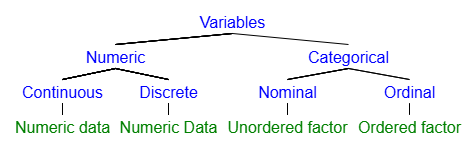
\includegraphics[keepaspectratio]{data_types.png}}

}

\caption{A hierarchy of variables and their corresponding R data types}

\end{figure}%

For our last bit, let's learn a little about working with functions that
don't come included in base R.

\chapter{Packages and the Tidyverse}\label{packages-and-the-tidyverse}

R's open-source culture has encouraged a rich ecosystem of custom
functions designed by scientists and researchers in the R userbase.
These come in the form of `packages', which are suites of several
related functions. For example, there are packages for conducting
statistical tests, producing data visualizations, generating
publication-ready tables, and all manner of other tasks.

\section{Loading Packages}\label{loading-packages}

Let's try this out with one of the better known R packages--`tidyverse'.
This is actually a collection of several packages with a variety of
interrelated functions for `tidying', visualizing, and analyzing data.
We will focus on what we need from `tidyverse', but, if you're curious,
you can read more here: \url{https://www.tidyverse.org/}

If you're on a lab computer, this package may already be installed.
Let's check by running the following command:

\begin{Shaded}
\begin{Highlighting}[]
\FunctionTok{library}\NormalTok{(tidyverse)}
\end{Highlighting}
\end{Shaded}

\begin{verbatim}
-- Attaching core tidyverse packages ------------------------ tidyverse 2.0.0 --
v dplyr     1.1.4     v readr     2.1.5
v forcats   1.0.0     v stringr   1.5.1
v ggplot2   3.5.2     v tibble    3.3.0
v lubridate 1.9.4     v tidyr     1.3.1
v purrr     1.1.0     
-- Conflicts ------------------------------------------ tidyverse_conflicts() --
x dplyr::filter() masks stats::filter()
x dplyr::lag()    masks stats::lag()
i Use the conflicted package (<http://conflicted.r-lib.org/>) to force all conflicts to become errors
\end{verbatim}

If you receive an error when you run this, you likely do not have the
package installed on your system. This is also probably the case if you
are on your personal device and only recently acquired R.

If you got an error, run the following command:

\begin{Shaded}
\begin{Highlighting}[]
\FunctionTok{install.packages}\NormalTok{(}\StringTok{"tidyverse"}\NormalTok{)}
\end{Highlighting}
\end{Shaded}

With a few exceptions, you will always install new packages in this
fashion: install.packages(``package\_name'')

After it's done installing, go back and run the library(tidyverse)
command again. Note that you always need to do this for an added
package. Whether you've had it for a while or just installed it, you
need to load any outside package into your current session by placing
its name in the library() function.

\begin{Shaded}
\begin{Highlighting}[]
\FunctionTok{library}\NormalTok{(tidyverse)}
\end{Highlighting}
\end{Shaded}

\section{Practice with Data
Manipulation}\label{practice-with-data-manipulation}

Let's try bringing in a data frame to play with a few tidyverse
functions. We'll use the load() function to bring in a subset of the
General Social Survey, which contains a few variables from the 2022
survey wave. Run the following command and select the file
``gss\_sub.rda''

\begin{Shaded}
\begin{Highlighting}[]
\FunctionTok{load}\NormalTok{(}\FunctionTok{file.choose}\NormalTok{())}
\end{Highlighting}
\end{Shaded}

The file.choose() function will open up a file-explorer window that
allows you to manually select an R data file to load in. We'll talk
about some other ways to import data files using R syntax next time.

\part{Day 2: Survey Data and Univariate Analysis}

\part{Day 3: Bivariate Analysis with the GSS}

\part{Day 4: Multivariable Analysis and Elaboration}

\part{Day 5: Data Visualization and ggplot}




\end{document}
